\documentclass{article}


\usepackage{arxiv}

\usepackage[utf8]{inputenc} % allow utf-8 input
\usepackage[T1]{fontenc}    % use 8-bit T1 fonts
\usepackage{hyperref}       % hyperlinks
\usepackage{url}            % simple URL typesetting
\usepackage{booktabs}       % professional-quality tables
\usepackage{amsfonts}       % blackboard math symbols
\usepackage{nicefrac}       % compact symbols for 1/2, etc.
\usepackage{microtype}      % microtypography
\usepackage{graphicx}
\usepackage{natbib}
\usepackage{doi}

\usepackage{amsmath}
\usepackage{nicematrix}
\usepackage{cleveref}
\usepackage{listings}
\usepackage{pgfplots}

\usepackage{algpseudocode}
\usepackage{algorithm}

\renewcommand{\algorithmicrequire}{\textbf{Input:}}
\renewcommand{\algorithmicensure}{\textbf{Initialize:}}


\NiceMatrixOptions{cell-space-top-limit=5pt,cell-space-bottom-limit=5pt,columns-width=20pt}

\crefname{lstlisting}{listing}{listings}
\Crefname{lstlisting}{Listing}{Listings}


% Listing options
\definecolor{codegreen}{rgb}{0,0.6,0}
\definecolor{codegray}{rgb}{0.5,0.5,0.5}
\definecolor{codepurple}{rgb}{0.58,0,0.82}
\definecolor{backcolour}{rgb}{0.95,0.95,0.92}

\lstdefinestyle{python_style}{
    backgroundcolor=\color{backcolour},
    commentstyle=\color{codegreen},
    keywordstyle=\color{magenta},
    numberstyle=\tiny\color{codegray},
    stringstyle=\color{codepurple},
    basicstyle=\ttfamily\footnotesize,
    breakatwhitespace=false,
    breaklines=true,
    captionpos=b,
    keepspaces=true,
    numbers=left,
    numbersep=5pt,
    showspaces=false,
    showstringspaces=false,
    showtabs=false,
    tabsize=2
}
\lstset{style=python_style}

\def\R{\mathbb{R}}


\title{Recommendation systems via approximate matrix factorization}

%\date{September 9, 1985}	% Here you can change the date presented in the paper title
\date{} 					% Or removing it

\author{
  \hspace{1mm}Dmitry Beresnev \\
	AIDS-MS1, Innopolis University\\
	\texttt{d.beresnev@innopolis.university} \\
	\And{}
  \hspace{1mm}Vsevolod Klyushev \\
	AIDS-MS1, Innopolis University\\
	\texttt{v.klyushev@innopolis.university}
}

\renewcommand{\undertitle}{\textbf{Group 1} Report for HDDA F24 course}
\renewcommand{\headeright}{}

\begin{document}
\maketitle


\section{Introduction}

\subsection{Problem formulation}


We were given the following problem:
\begin{equation}\label{eq:problem}
  \min_{U \in \R^{m \times r}, V \in \R^{r \times n}} \|W \circ (X - UV)\|^2_F
\end{equation}
where $X \in \R^{m \times n} $ --- target matrix, $W \in \R^{m \times n} $ --- binary matrix (0 or 1), $r \in \R_+$ --- rank of factorization.

\subsection{Initialization of $U,V$}

In order to have a good starting point, we decided to do the following:
\begin{itemize}
  \item Impute unknown cells in matrix with mean among movies (via sklearn SimpleImputer)
  \item Perform randomized SVD decomposition (via sklearn randomized SVD) with required rank
  \item Take necessary number of first and last components of decomposition as $U$ and $V$ matrices correspondingly
\end{itemize}

\section{Notations}

 {
  \renewcommand{\arraystretch}{1.5}
  \renewcommand{\tabcolsep}{10pt}
  \begin{table}[hbthbt]
    \centering
    \begin{tabular}{cc}
      \toprule
      \textbf{Notation}              & \textbf{Meaning}                                          \\
      \midrule
      $\langle \cdot, \cdot \rangle$ & dot product (Frobenius inner product in case of matrices) \\
      $\| \cdot \|$                  & second norm (Frobenius norm in case of matrices)          \\
      $f, f(\cdot)$                  & objective function                                        \\
      $\nabla f, \nabla f(\cdot)$    & gradient of objective function                            \\
      $X_i$                          & $i$-th column of matrix $X$                               \\
      $X^\top_i$                     & $i$-th row of matrix $X$                                  \\
      \bottomrule
    \end{tabular}
  \end{table}
 }

\section{Gradient Descent}\label{sec:gradient_descent}

\subsection{Gradients derivation}

In order to use Gradient Descent method \Cref{algo:gd}, we need to compute gradients with respect to each parameter $U$ and $V$.
Using matrix-vector differentiation rules and some help from~\cite{kwan}, we obtained the following:
\begin{equation}\label{eq:grads}
  \begin{aligned}
     & \cfrac{\partial \|W \circ (X - UV)\|^2_F}{\partial U} = -2 (W \circ X) V^T + 2 (W \circ (UV)) V^T \\
     & \cfrac{\partial \|W \circ (X - UV)\|^2_F}{\partial V} = -2 U^T (W \circ X) + 2 U^T (W \circ (UV)) \\
  \end{aligned}
\end{equation}

\begin{algorithm}[H]
  \caption{Gradient Descent optimizer}\label{algo:gd}
  \begin{algorithmic}[0]
    \Require{$\theta_0$ (parameters to optimize), $f(\theta)$ (objective function), $\mathcal{L}(p)$ (step size choosing strategy) }

    \For{$t = 1$ \textbf{to} $\dots$}
    \State{$p_t \gets -\nabla_{\theta}f_t(\theta_{t-1}) $} \Comment{Step direction}
    \State{Choose step size $\gamma$ according to $\mathcal{L}(p_t)$}
    \State{$\theta_t \gets \theta_{t-1} + \gamma p_t $}
    \EndFor{}

    \State{\Return{$\theta_t$}}

  \end{algorithmic}
\end{algorithm}

We have also added the regularization, so the final problem is
\begin{equation}\label{eq:problem_reg}
  \min_{U \in \R^{m \times r}, V \in \R^{r \times n}} \|W \circ (X - UV)\|^2_F + \lambda\|U\|^2_F + \lambda\|V\|^2_F
\end{equation}
where $\lambda$ --- regularization parameter.

Finally, gradients of \Cref{eq:grads} is computed as
\begin{equation}\label{eq:grads_reg}
  \begin{aligned}
     & \cfrac{\partial (\|W \circ (X - UV)\|^2_F + \lambda\|U\|^2_F + \lambda\|V\|^2_F)}{\partial U} = -2 (W \circ X) V^T + 2 (W \circ (UV)) V^T + 2\lambda U \\
     & \cfrac{\partial (\|W \circ (X - UV)\|^2_F + \lambda\|U\|^2_F + \lambda\|V\|^2_F)}{\partial V} = -2 U^T (W \circ X) + 2 U^T (W \circ (UV)) + 2\lambda V \\
  \end{aligned}
\end{equation}

The overall method is then the following: on each iteration we:
\begin{enumerate}
  \item Fix $V$ and update $U$ using the first equation of \Cref{eq:grads_reg} and \Cref{algo:gd}
  \item Fix $U$ and update $V$ using the second equation of \Cref{eq:grads_reg} and \Cref{algo:gd}
\end{enumerate}

Since the objective function is $f : \R^{m \times n}  \rightarrow \R $, the gradients are  matrices.
However, some step sizes strategies and optimizers uses dot product (for example, between descent direction and gradient). Therefore, hereafter, we substitute, where it is necessary, vector dot product with Frobenius inner product, defined as:
\begin{equation}\label{eq:frob}
  \langle A, B \rangle_F = Tr (A^T B)
\end{equation}

\subsection{Step size strategies}

We decided to test different strategies for finding the decent step size $\alpha$.

\paragraph{Constant step size}
\begin{equation*}
  \alpha_k = \alpha
\end{equation*}

\paragraph{Decreasing step size}
\begin{equation*}
  \alpha_k = \frac{1}{k}
\end{equation*}
or, alternatively,
\begin{equation*}
  \alpha_k = \frac{1}{\sqrt{k}}
\end{equation*}

\paragraph{Estimation of Lipschitz constant}
We know that for $L$-smooth function $f$, the following holds:
\begin{equation*}
  \|\nabla f(x) -\nabla f(y)\| \leq L  \|x -  y\|, \forall x,y
\end{equation*}

Also, we know that in case of $L$-smooth function, the optimal step size would be $\alpha_k = \frac{1}{L}$.
Hence, we can try to iteratively estimate it, what is done in \Cref{algo:lr_est}.

\paragraph{Armijo rule}

A step length $\alpha$ is said to satisfy the Armijo condition, restricted to the descent direction $p$ ($p^T \nabla f(x) < 0$) if the following holds:
\begin{equation}\label{eq:armijo}
  f(x + \alpha p) \leq f(x) + c_1 \alpha \langle p, \nabla f(x) \rangle
\end{equation}
where $c_1 > 0$ is typically small (about 0.01) constant.

The Armijo rule ensures the `sufficient' decrease in the function after making a step (\Cref{fig:armijo}).
Hence, \Cref{algo:lr_armijo} iteratively decreases step size until it satisfies the Armijo condition.


\paragraph{Weak Wolfe conditions}
A step length $\alpha$ is said to satisfy the curvature condition, restricted to the descent direction $p$ if the following holds:
\begin{equation}\label{eq:curv}
  - \langle p, \nabla f(x + \alpha) \rangle \leq -c_2 \langle p, \nabla f(x) \rangle
\end{equation}
where $c_2 > 0$.
The curvature condition helps to find points, in which our function is not decreasing as fast as in starting point \Cref{fig:curvature}.



A step length $\alpha$ is said to satisfy the (Weak) Wolfe conditions (\Cref{fig:weak_wolfe}) with $c_2 > c_1 > 0$, if both \Cref{eq:armijo,eq:curv} holds. Therefore, we can iteratively decrease step size until it satisfies the Weak Wolfe conditions. In \cite{evgrafov} the efficient bisection algorithm (\Cref{algo:lr_biwolfe}) for such procedure is presented.


\paragraph{Strong Wolfe conditions}
However, the Wolfe conditions can result in a value for the step length that is not close to a minimizer of $\phi(\alpha) = f(x + \alpha p)$. We can modify the curvature condition as following:
\begin{equation}\label{eq:curv_strong}
  \| \langle p, \nabla f(x + \alpha) \rangle \| \leq c_2 \| \langle p, \nabla f(x) \rangle \|
\end{equation}

A step length $\alpha$ is said to satisfy the Strong Wolfe conditions (\Cref{fig:strong_wolfe}) with $c_2 > c_1 > 0$, if both \Cref{eq:armijo,eq:curv_strong} holds.These conditions force $\alpha$ to lie close to a critical point of $\phi$. The algorithm that searches for points satisfying the String Wolfe Conditions is presented in \Cref{algo:lr_wolfe}.

\subsection{Optimizers}

We have also decided to try other optimizer rather than only Gradient Descent. New optimization algorithms can help to improve the convergence and avoid local minima by introducing either the idea of momentum (\Cref{algo:hb,algo:nesterov}), or adaptivity (\Cref{algo:lr_adaptive,algo:adagrad,algo:rmsprop,algo:adam}).

\paragraph{Adaptive gradient descent}
Relatively new approach, proposed in 2020 in paper~\cite{malitsky}, which is more the step size search approach, than the true optimizer. This method has several advantages:
\begin{itemize}
  \item It is not iterative
  \item It relies on local smoothness (as a method of estimating $\frac{1}{L}$)
\end{itemize}.
In a nutshell, the algorithm \Cref{algo:lr_adaptive} at each iteration $k$ tries to find the maximum step size $\alpha_k$ satisfying
\begin{equation}\label{eq:adaptive}
  \begin{aligned}
     & \frac{\alpha^2_k}{\alpha^2_{k-1}} \leq (1+\theta_{k-1})                        \\
     & \alpha_k \leq \frac{\|x^k - x^{k-1} \|}{2 \|\nabla f(x^k) - \nabla f(x^{k-1})} \\
  \end{aligned}
\end{equation}
where $\theta_k = \frac{\alpha_k}{\alpha_{k-1}}$.

The first inequality of \Cref{eq:adaptive} makes sure new step size not to be too big compared to previous. The second inequality of \Cref{eq:adaptive} sets upper bound for step to be $\frac{1}{2L}$, where $L$ is that the smoothness condition holds for the current and the precious points.


\paragraph{Heavy Ball}
In theory is usually written as
\begin{align*}
   & x_{k+1} = x_k - \alpha_k  \nabla f(x_k) + \beta_k (x_k - x_{k-1})
\end{align*}
where $\beta$ --- momentum, which determines the effect of the previous steps on the current update.

The Heavy Ball method was proposed in 1964 by Boris Polyak. This is a classic improvement of the standard Gradient Descent by adding momentum: the method combines the current gradient with the previous history to accelerate convergence.

Realization is presented in \Cref{algo:hb}.

\paragraph{Nesterov momentum}
In theory is usually written as
\begin{align*}
   & x_{k+1} = y_k - \alpha_k  \nabla f(y_k)     \\
   & y_{k+1} = x_{k+1} + \beta_k (x_{k+1} - x_k)
\end{align*}
where $\beta_k$ --- momentum, usually taken constant $\beta_k = \beta$ .

The Nesterov Accelerated Method extends the idea of momentum in Gradient Descent. It was introduced by Yuri Nesterov in 1983. The basic idea is to use partial prediction when updating parameters, including momentum to accelerate convergence. The key difference from the heavy ball method is that due to the impulse to the gradient counting point, extrapolation, or `looking into the future' occurs.

Realization is presented in \Cref{algo:nesterov}.

\paragraph{AdaGrad}
\begin{align*}
   & g_k = \nabla f(x_k)                                       \\
   & G_k = G_{k-1} + g_k^2                                     \\
   & x_{k+1} = x_k - \frac{\gamma_k}{\sqrt{G_k}+ \epsilon} g_k
\end{align*}
where $G_k$ --- cumulative squared sum of gradients, $\epsilon$ --- small constant for stability.

AdaGrad was developed to solve the problems associated with setting a uniform learning rate for all parameters, especially in situations where the features have significantly different frequency or importance: it would be good to be able to update the parameters with an eye to how typical a feature they capture.

Realization is presented in \Cref{algo:adagrad}.

\paragraph{RMSprop}
\begin{align*}
   & g_k =  \nabla f(x_k)                                       \\
   & G_k = \beta G_{k-1} + (1-\beta) g_k^2                      \\
   & x_{k+1} = x_k - \frac{\gamma_k}{\sqrt{G_k} + \epsilon} g_k
\end{align*}
where $G_k$ --- weighted moving average of squared gradients.

The key idea of RMSProp is to scale the gradient of each weight in the model by dividing it by the root mean square value of the gradients of that weight. This helps prevent weights with high gradients from learning too quickly, while at the same time allowing weights with low gradients to continue learning faster. Method solves the main problem of AdaGrad --- old gradients and recent gradients have different weights, that is, there is a kind of `forgetting' of history.

Realization is presented in \Cref{algo:rmsprop}.


\paragraph{Adam}
\begin{align*}
   & g_k =  \nabla f(x_k)                                                   \\
   & m_k = \beta_1 m_{k-1} + (1-\beta_1) g_k                                \\
   & v_k = \beta_2 v_{k-1} + (1-\beta_2) g_k^2                              \\
   & \hat{m_k} = \frac{m_k}{1-\beta_1^k}                                    \\
   & \hat{v_k} = \frac{v_k}{1-\beta_2^k}                                    \\
   & x_{k+1} = x_k - \frac{\gamma_k}{\sqrt{\hat{v_k}} + \epsilon} \hat{m_k}
\end{align*}
where $m_k, v_k$ --- so called first and second momentum of gradient.

Adam supports exponential moving averages of weights and gradients, which it uses to scale the learning rate: it uses estimates of the mean and variance of gradients to adaptively scale the learning rate during training.

If we consider the following type of formula for correction ($\hat{v_k}$):
$$
  \hat{v_k} = \frac{(1-\beta_2)\sum_{i=1}^k \beta_2^{k-i} \text{diag}(g_i \odot g_i)}{1 - \beta_2^k}.
$$
one can notice that $g_k^2$ is taken with a weight of $1$, $g_{k-1}^2$ is taken with a weight of $\beta_2$, $g_{k-2}^2$ is taken with a weight of $\beta_2^2$, and so on.
Next, all weights are divided by $1+\beta_2+\beta_2^2+\dots+\beta_2^k = \frac{1 - \beta_2^k}{(1-\beta_2)}$. Thus, the sum of all the weights is equal to 1, that is, a convex combination is obtained.
Therefore, the weights for the gradients depend on the iteration number. In the initial iterations, it behaves in a similar way to AdaGrad, and in the later iterations it becomes similar to RMSprop.

Realization is presented in \Cref{algo:adam}.

\paragraph{BFGS}
The Broyden–Fletcher–Goldfarb–Shanno (BFGS) algorithm is a quasi-Newton method, that approximates the Hessian $B_k$ of the objective function. The authors suggest to compute $H_k = B^{-1}_k$ by solving
\begin{equation}\label{eq:bfgs}
  \begin{aligned}
                 & \min_H \| H_k - H \| \\
    \text{s.t. } & H = H^{\top}         \\
                 & H y_k = s_k          \\
  \end{aligned}
\end{equation}
where $y_k = \nabla f(x_{k+1}) - \nabla f(x_k)$ and $s_k = x_{k+1} - x_k$.

The suggestion is quite intuitive: let us look for the $H_k$ that is closest in any norm to the real inverse Hessian, satisfies the quasi-Newtonian equation (last equality in \Cref{eq:bfgs}) and is symmetric (like the real inverted Hessian itself).

The authors proved that a two-rank Hessian update is enough:
\begin{equation*}
  B_{k+1} = B_k + \alpha uu^T + \beta v v^T
\end{equation*}

And one can obtain the equation for the inverted hessian:
\begin{equation*}
  H_{k+1} = (I - \rho_k  s_ky^{\top}_k)H_k(I - \rho_k  y_k s^{\top}_k) +\rho_k  s_k s^{\top}_k,
\end{equation*}
where $\rho_k = \dfrac{1}{y^{\top}_k s_k}$.

Realization is presented in \Cref{algo:bfgs}.

Note, that we can not directly use BFGS for the methods \Cref{eq:problem,eq:problem_reg}, because the approximated hessian (and its inverse) would be tensors as second derivatives of function $f: \R^{m \times n} \rightarrow \R $. However, this methods can be used for \Cref{sec:vec}.

\section{Vector Gradient Descent}\label{sec:vec}
Instead of making update for entire $U$ or $V$ simultaneously, we can make updates row by row (column by column for $V$). The reasons are the following:
\begin{enumerate}
  \item The objective function becomes $f: \R^d \rightarrow \R$, so we can apply methods like BFGS (\Cref{algo:bfgs})
  \item There will be more updates, and such updates will be more diverse: we will use just updated values for new updates
\end{enumerate}

Therefore, the new problem with fixed $V$ becomes
\begin{equation}\label{eq:vec_u}
  \min_{U^\top_i \in \R^r} \|W^\top_i \circ (X^\top_i - U^\top_i V)\|^2 + \lambda\|U^\top_i\|^2, \text{ }\forall i \in \{1,2,\ldots,m\}
\end{equation}
and the new problem with fixed $U$:
\begin{equation}\label{eq:vec_v}
  \min_{V_j \in \R^r} \|W_j \circ (X_j - UV_j)\|^2  + \lambda\|V_j\|^2, \text{ }\forall j \in \{1,2,\ldots,n\}
\end{equation}

Hence gradient of \Cref{eq:vec_u} is
\begin{equation}\label{eq:vec_grads_u}
  \cfrac{\partial (\|W^\top_i \circ (X^\top_i - U^\top_i V)\|^2 + \lambda\|U^\top_i\|^2)}{\partial U^\top_i} = -2 (W^\top_i \circ X^\top_i) V^T + 2 (W^\top_i \circ (U^\top_i V)) V^T + 2\lambda U^\top_i
\end{equation}
and the gradient of \Cref{eq:vec_v}:
\begin{equation}\label{eq:vec_grads_v}
  \cfrac{\partial (\|W_j \circ (X_j - UV_j)\|^2  + \lambda\|V_j\|^2)}{\partial V_j} =  -2 U^T (W_j \circ X_j) + 2 U^T (W_j \circ (UV_j)) + 2\lambda V_j
\end{equation}

Obviously, if we want to obtain more diverse updates, we should change the order of $U$ and $V$ updates: if we firstly update all rows of $U$ and only then all the columns of $V$, the updates would be the same as in \Cref{eq:grads_reg}.

Remember, $X \in \R^{m \times n}$, what means that number of rows of $U$ and number of columns of $V$ has the ratio $\frac{m}{n} \approx \frac{k_U}{k_V}$, where $k_U$ and $k_V$ are possibly small integers. Therefore,it is reasonable to firstly update $k_U$ rows of $U$ and then update $k_V$ columns of $V$.
For the given problem, $X \in \R^{6040 \times 3952}$, so $k_U \approx 3$ and $k_V \approx 2$
The final algorithm, what we called Vector Gradient Descent, then looks as presented in \Cref{algo:vec_grad}.

\begin{algorithm}[H]
  \caption{Vector Gradient Descent}\label{algo:vec_grad}
  \begin{algorithmic}[0]
    \Require{$X, W \in \R^{m \times n}$ --- given initial and binary matrices,
      $U \in \R^{m \times r}, V \in \R^{r \times n}$ --- arbitrary matrices,
      $k_U$, $k_V$ --- small integers such that $\frac{m}{n} \approx \frac{k_U}{k_V}$}
    \State{}
    \State{$d \gets k_U + k_V $}
    \Repeat
    \For{$t = 0$ \textbf{to} $n+m-1$}
    \State{$r \gets t \textbf{ mod } d $}
    \If{$r < k_U$}
    \State{$i \gets k_U \cdot (t \textbf{ div } d) + r +1 $}
    \If{$i > m$}
    \State{\textbf{continue}}
    \EndIf{}
    \State{Update $U^\top_i$ using \Cref{eq:vec_grads_u}}
    \Else{}
    \State{$j \gets k_V \cdot (t \textbf{ div } d) + r - k_U +1 $}
    \If{$j > n$}
    \State{\textbf{continue}}
    \EndIf{}
    \State{Update $V_j$ using \Cref{eq:vec_grads_v}}
    \EndIf{}
    \EndFor{}
    \Until{convergence}
    \State{}
    \State{\Return{$U,V$}}
  \end{algorithmic}
\end{algorithm}

\section{Non-Negative Matrix Factorization (NNMF)}\label{sec:NNMF}

Let us add to the initial problem (\Cref{eq:problem}) non-negativity constraints:
\begin{equation}\label{eq:nnmf_problem}
  \begin{aligned}
                 & \min_{U \in R^{m\times r}, V \in R^{r\times n}} \|W \circ (X - UV)\|^2_F \\
    \text{s.t. } & U, V \geq 0                                                              \\
  \end{aligned}
\end{equation}

In order to solve such problem more easily, we need to derive multiplicative updates for $U$ and $V$.

Firstly, let us recall gradient update from the previous parts:

\begin{equation}
  U \gets U + \alpha_u ((W \circ X) V^T - (W \circ (UV)) V^T)
\end{equation}

If we set $\alpha_u = \cfrac{U}{((W \circ (UV)) V^T)}$, we get:

\begin{equation}
  \begin{aligned}
    U & \gets U + \alpha_u ((W \circ X) V^T - (W \circ (UV)) V^T) = \\ & = U + U \circ \cfrac{((W \circ X) V^T)}{((W \circ (UV)) V^T)} - U \circ \cfrac{((W \circ (UV)) V^T)}{((W \circ (UV)) V^T)} = \\ & = U + U \circ \cfrac{((W \circ X) V^T)}{((W \circ (UV)) V^T)} - U =\\ & = U \circ \cfrac{((W \circ X) V^T)}{((W \circ (UV)) V^T)}
  \end{aligned}
\end{equation}

We have achieved multiplicative update for $U$. Now, let us do the same for $V$:

\begin{equation}
  V \gets V + \alpha_v (U^T (W \circ X) - U^T (W \circ (UV)))
\end{equation}

If we'll use $\alpha_v = \cfrac{V}{(U^T (W \circ (UV)))}$, then we'll get:

\begin{equation}
  \begin{aligned}
    V & \gets V + \alpha_v (U^T (W \circ X) - U^T (W \circ (UV))) = \\ & = V + V \circ \cfrac{(U^T (W \circ X))}{(U^T (W \circ (UV)))} - V \circ \cfrac{(U^T (W \circ (UV)))}{(U^T (W \circ (UV)))} = \\ & = V + V \circ \cfrac{(U^T (W \circ X))}{(U^T (W \circ (UV)))} - V = \\ & = V \circ \cfrac{(U^T (W \circ X))}{(U^T (W \circ (UV)))}
  \end{aligned}
\end{equation}

Now we also have achieved multiplicative update for $V$.

Such idea was used in Lee and Seung paper~\cite{lee} for problem without mask in order to avoid subtraction, so the production of negative elements. Authors provided the proof of convergence for such adaptive learning rates for problems without mask.

However, our binary mask $W$ brings some problems with division operation (the division on zero or very small number is possible). Adding some small constant $\epsilon$ to denominator captures this. This brings our multiplicative updates to be in the following forms:

\begin{equation}
  U \gets U \circ \cfrac{((W \circ X) V^T)}{((W \circ (UV)) V^T + \epsilon)}
\end{equation}
\begin{equation}
  V \gets V \circ \cfrac{(U^T (W \circ X))}{(U^T (W \circ (UV)) + \epsilon)}
\end{equation}

However, results demonstrated by such method is not satisfactory: it over-fits on the first iteration and shows very bad performance on test set (\Cref{fig:nnmf}).

\section{Neural Network}\label{sec:NN}
As an alternative approach we decided to train simple neural network with the following parameters:
\begin{itemize}
  \item 4 layers ($23\times64, 64\times128, 128\times64, 64\times1$)
  \item ReLU as activation function after each layer
  \item MSELoss criterion
  \item Adam optimizer with step size $\alpha = 0.001$
  \item Early stopping (if on test set loss is not decreasing for 3 iterations)
  \item Maximum number of training epochs $k= 50$
\end{itemize}

Model input consists of:
\begin{itemize}
  \item Min-max scaled `user\_id`
  \item Min-max scaled `movie\_id`
  \item One-hot encoded `genres` (we have 18 unique genres)
  \item Binary encoded `gender`
  \item Min-max scaled first two user features (`feature\_1` and `feature\_2`)
\end{itemize}

As output model returns just one number --- rating for specific pair of user and movie.

Model was able to achieve average MSE loss on test set $\approx 1.1$

\section{Results}
We have tested several approaches: Gradient descent (\Cref{sec:gradient_descent}), Vector Gradient descent (\Cref{sec:vec}), Non-Negative Matrix Factorization (\Cref{sec:NNMF}) and Neural Network (\cref{sec:NN}).

Both Neural Network and Vector Gradient descent showed their applicability for recommendation system task, however, they have been outperformed by other models.

As for NNMF, after several experiments we came to the conclusion, that such approach is inapplicable for recommendation system task mostly because of the mask in the problem formulation. Mask makes NNMF to set almost all unknown values to 1, which is quite a bad decision.

The Gradient descent method showed the best overall performance (both in terms of time and RMSE score on test data). Among all different optimizers, step selection strategies and other hyper-parameters (you can check experiments in \Cref{sec:experiments}) we found the best composition: Gradient descent method for $r=10$ with estimate 1/L strategy and $\lambda=2$. This method achieved RMSE score 0.86 on test data.

\bibliographystyle{plain}
\bibliography{references}


\clearpage
\appendix

\part*{Supplementary materials}

\section{Step Size Conditions Figures}

\begin{figure}[H]
  \centering
  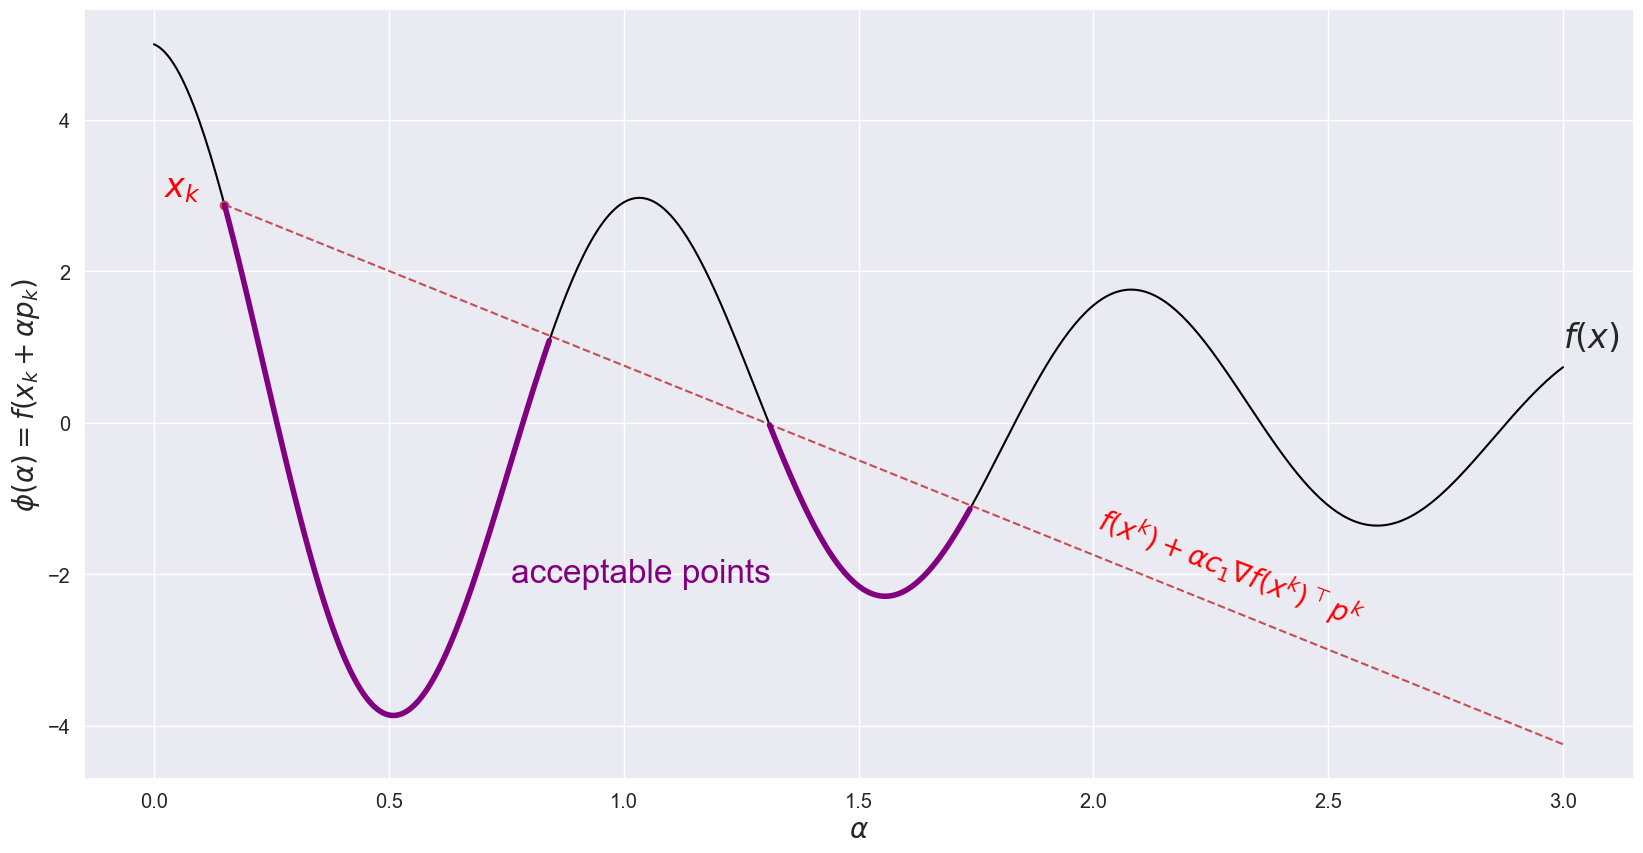
\includegraphics[width=\textwidth,keepaspectratio]{../data/armijo.png}
  \caption[Armijo rule]{Armijo rule}\label{fig:armijo}
\end{figure}

\begin{figure}[H]
  \centering
  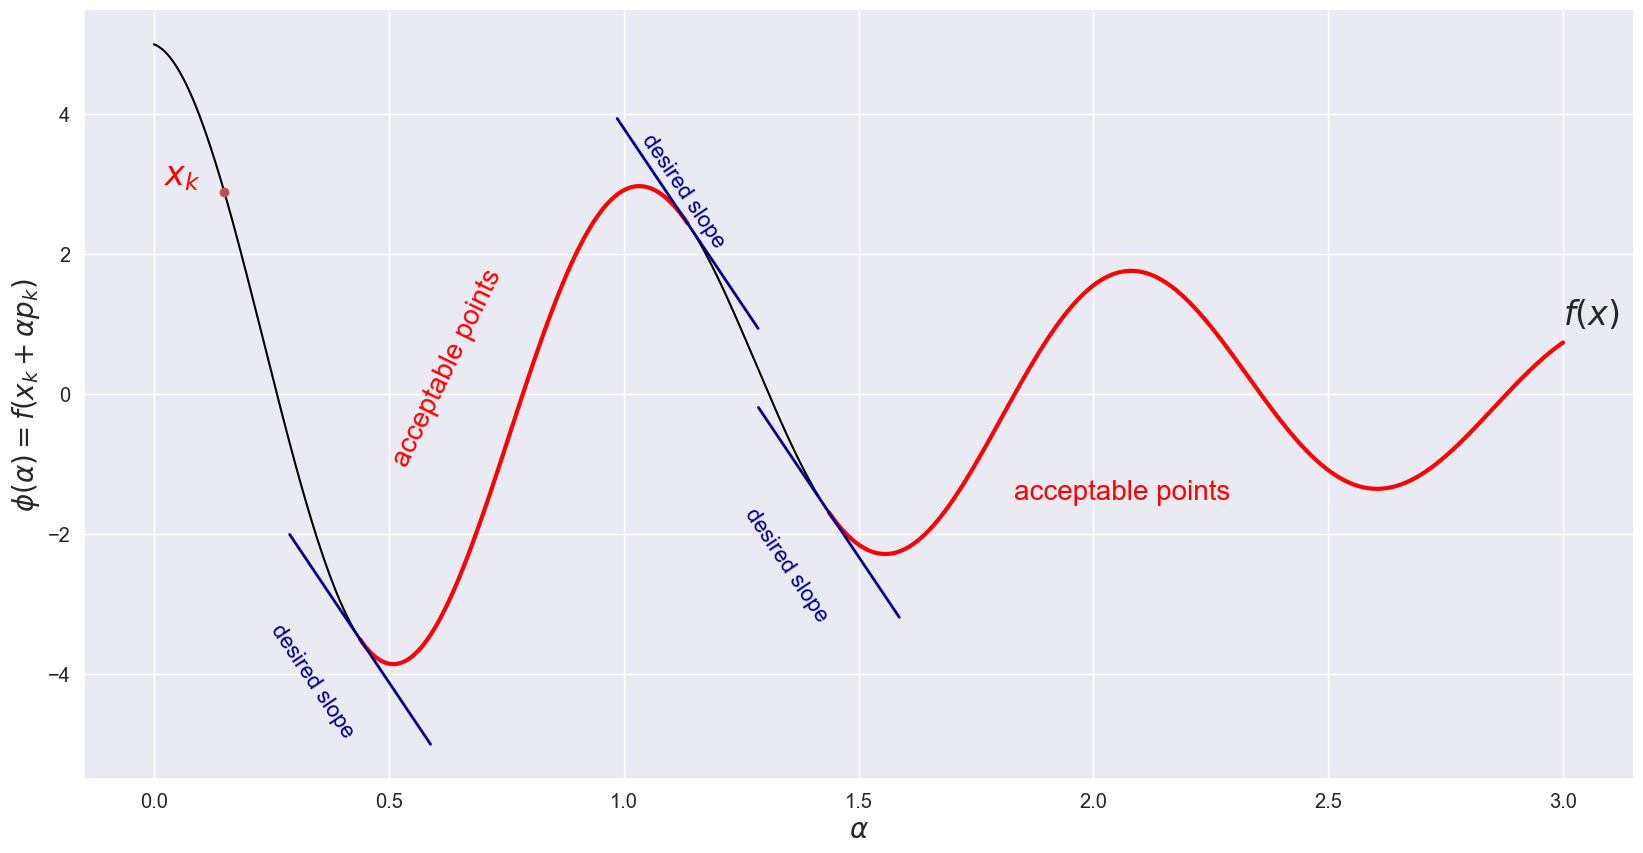
\includegraphics[width=\textwidth,keepaspectratio]{../data/curvature.png}
  \caption[Curvature condition]{Curvature condition}\label{fig:curvature}
\end{figure}

\begin{figure}[H]
  \centering
  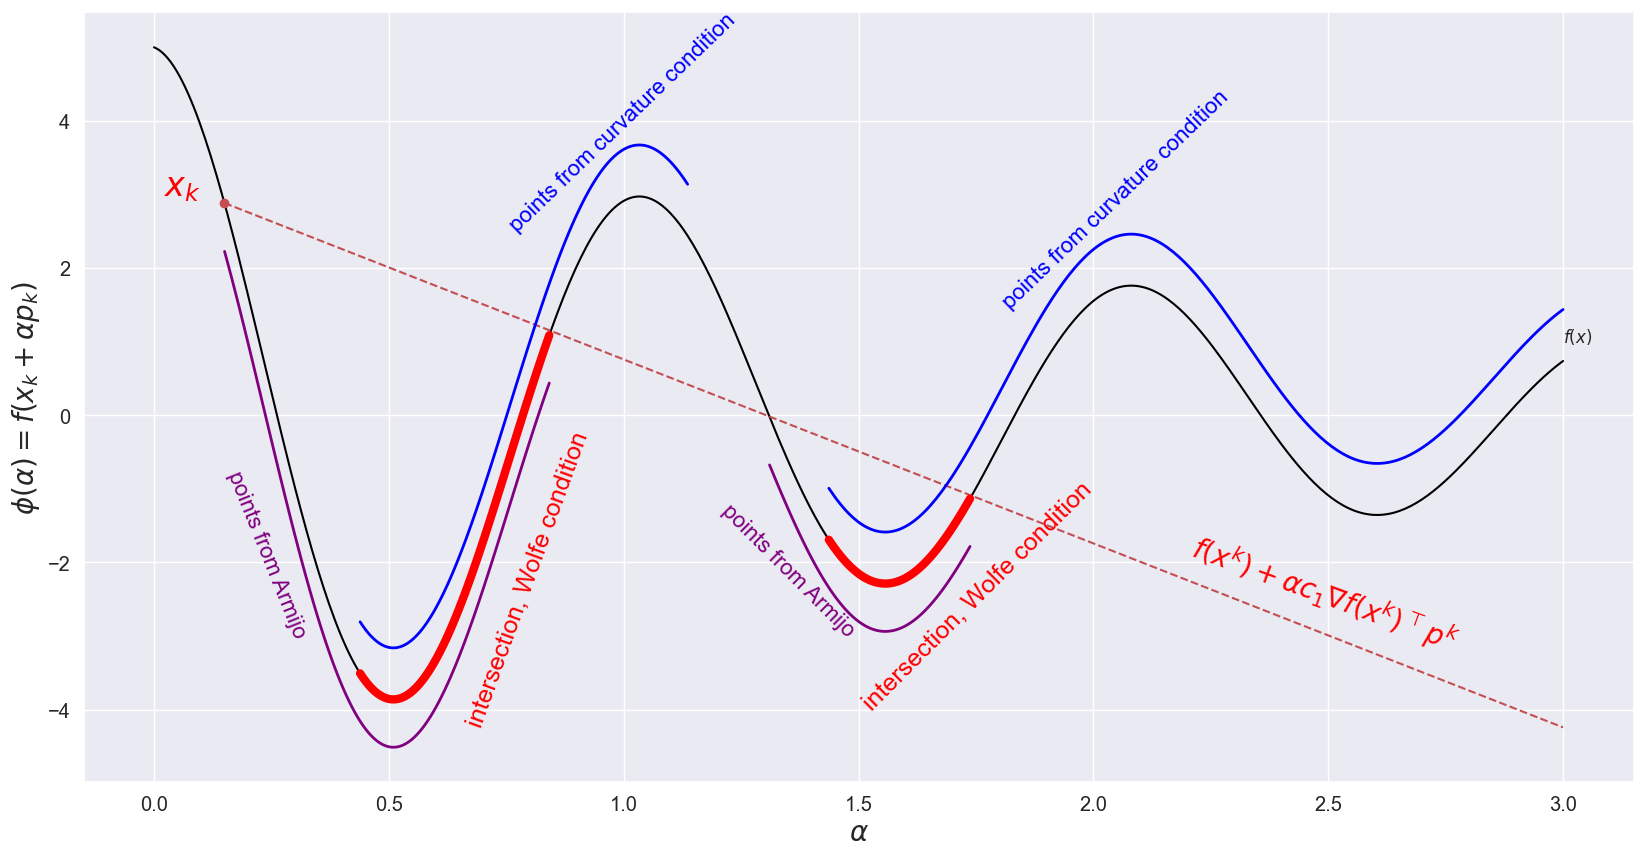
\includegraphics[width=\textwidth,keepaspectratio]{../data/weak_wolfe.png}
  \caption[Weak Wolfe conditions]{Weak Wolfe conditions}\label{fig:weak_wolfe}
\end{figure}

\begin{figure}[H]
  \centering
  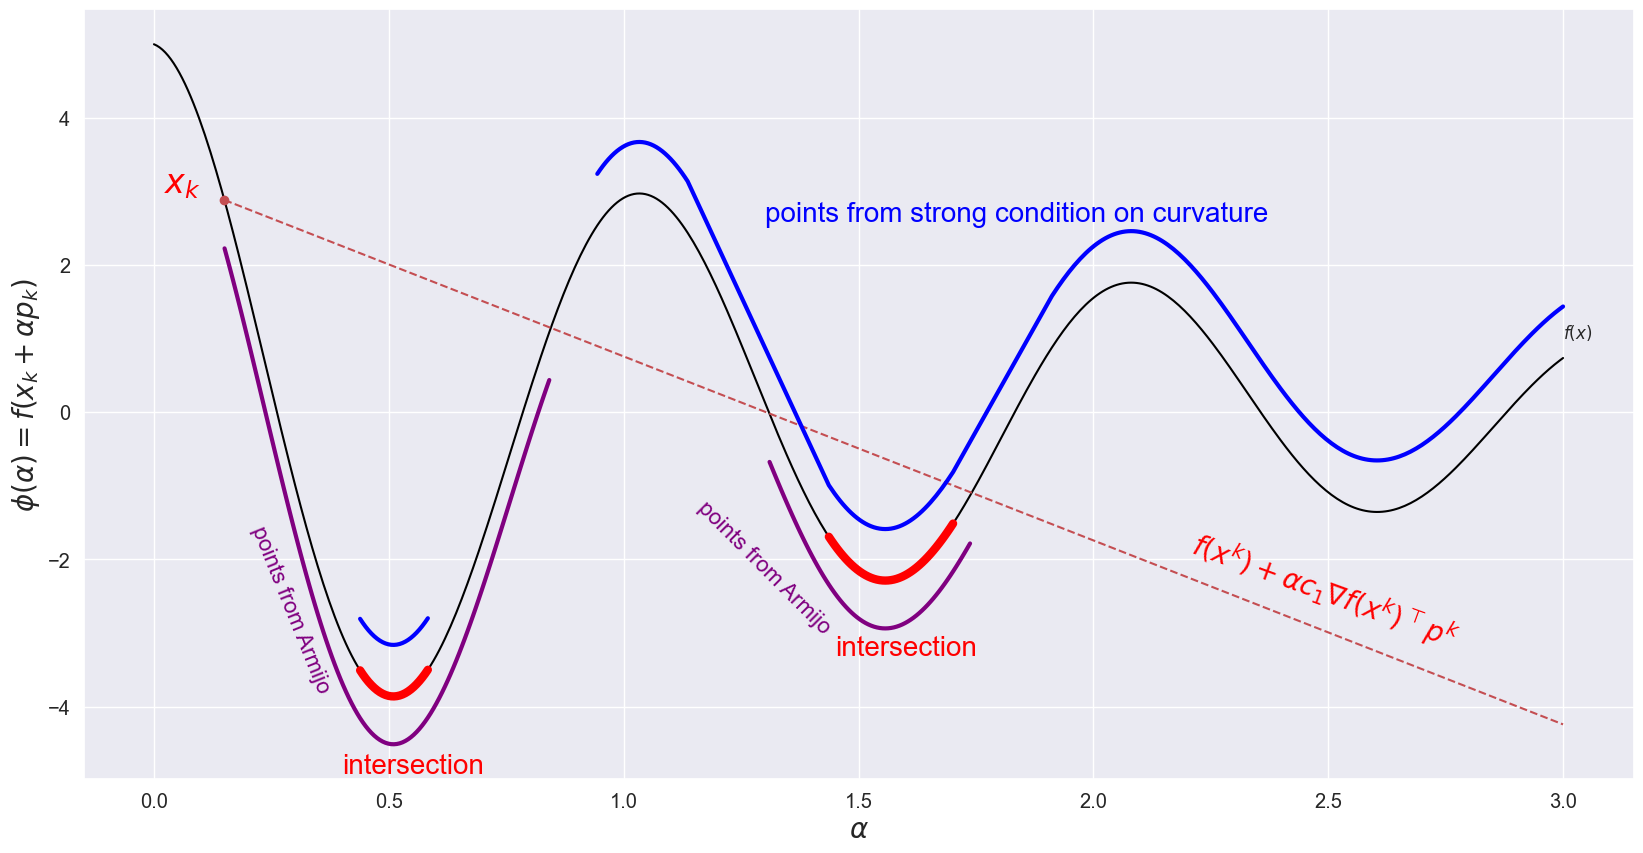
\includegraphics[width=\textwidth,keepaspectratio]{../data/strong_wolfe.png}
  \caption[Strong Wolfe conditions]{Strong Wolfe conditions}\label{fig:strong_wolfe}
\end{figure}

\section{Step selection Algorithms}

\begin{algorithm}[H]
  \caption{Estimate $1/L$}\label{algo:lr_est}
  \begin{algorithmic}[0]
    \Require{$\theta$ (point), $\nabla f(\theta)$ (gradient function), $p$ (desired direction), $\beta$ (multiplier), $t$ (max iterations) }

    \State{$\alpha \gets 1 $}
    \For{$i = 1$ \textbf{to} $t$}
    \State{$\theta_i \gets \theta + \alpha p $}
    \If{$\|\nabla f(\theta) -\nabla f(\theta_i)\| > \frac{1}{\alpha} \|\theta -  \theta_i\|$}
    \State{$\alpha \gets \beta \cdot \alpha$ }
    \If{$\alpha < \epsilon$}
    \State{\Return{$\alpha$}}
    \EndIf{}
    \Else{}
    \State{\Return{$\alpha$}}
    \EndIf{}
    \EndFor{}
    \State{\Return{$\alpha$}}

  \end{algorithmic}
\end{algorithm}

\begin{algorithm}[H]
  \caption{Armijo Step}\label{algo:lr_armijo}
  \begin{algorithmic}[0]
    \Require{$\theta$ (point), $f(\theta)$ (objective function), $p$ (desired direction), $\beta$ (multiplier), $c_1 > 0$, $t$ (max iterations) }

    \State{$\alpha \gets 1 $}
    \For{$i = 1$ \textbf{to} $t$}
    \State{$\theta_i \gets \theta + \alpha p $}
    \If{$f(\theta_i) > f(\theta) + c_1 \alpha \langle \nabla_{\theta} f(\theta), p \rangle $}
    \State{$\alpha \gets \beta \cdot \alpha$ }
    \If{$\alpha < \epsilon$}
    \State{\Return{$\alpha$}}
    \EndIf{}
    \Else{}
    \State{\Return{$\alpha$}}
    \EndIf{}
    \EndFor{}
    \State{\Return{$\alpha$}}

  \end{algorithmic}
\end{algorithm}

\begin{algorithm}[H]
  \caption{Bisection Weak Wolfe Step}\label{algo:lr_biwolfe}
  \begin{algorithmic}[0]
    \Require{$\theta$ (point), $f(\theta)$ (objective function), $p$ (desired direction), $\beta$ (multiplier), $c_1>0$, $c_2 >c_1$, $t$ (max iterations) }

    \State{$\alpha \gets 1 $}
    \State{$a \gets 0 $}  \Comment{Lower bound}
    \State{$b \gets +\infty $}  \Comment{Upper bound}
    \For{$i = 1$ \textbf{to} $t$}
    \State{$\theta_i \gets \theta + \alpha p $}

    \If{$f(\theta_i) > f(\theta) + c_1 \alpha \langle \nabla_{\theta} f(\theta), p \rangle$} \Comment{Armijo condition}

    \State{$b \gets \alpha$ }
    \State{$\alpha \gets \frac{1}{2} (a+b)$ } \Comment{Decrease step}

    \ElsIf{$\langle p, \nabla_{\theta}f(\theta_i)  \rangle < c_2  \langle p, \nabla_{\theta}f(\theta)  \rangle $} \Comment{Curvature condition}
    \State{$a \gets \alpha$ }

    \If{$b= +\infty$}
    \State{$\alpha \gets 2a$}
    \Else{}
    \State{$\alpha \gets \frac{1}{2} (a+b)$ } \Comment{Increase step}
    \EndIf{}
    \Else{}
    \State{\Return{$\alpha$}}
    \EndIf{}
    \EndFor{}
    \State{\Return{$\alpha$}}

  \end{algorithmic}
\end{algorithm}


\begin{algorithm}[H]
  \caption{Strong Wolfe Step}\label{algo:lr_wolfe}
  \begin{algorithmic}[0]
    \Require{$\theta$ (point), $f(\theta)$ (objective function), $p$ (desired direction), $\beta$ (multiplier), $c_1>0$, $c_2 >c_1$, $t$ (max iterations) }

    \State{$\alpha \gets 1 $}
    \For{$i = 1$ \textbf{to} $t$}
    \State{$\theta_i \gets \theta + \alpha p $}
    \If{$\bigl(f(\theta_i) > f(\theta) + c_1 \alpha \langle \nabla_{\theta} f(\theta), p \rangle \bigr)$
      \textbf{or} $\bigl( \| \langle p, \nabla_{\theta}f(\theta_i)  \rangle  \| > c_2 \| \langle p, \nabla_{\theta}f(\theta)  \rangle \|  \bigr)$}
    \State{$\alpha \gets \beta \cdot \alpha$ }
    \If{$\alpha < \epsilon$}
    \State{\Return{$\alpha$}}
    \EndIf{}
    \Else{}
    \State{\Return{$\alpha$}}
    \EndIf{}
    \EndFor{}
    \State{\Return{$\alpha$}}

  \end{algorithmic}
\end{algorithm}


\section{Optimizer Algorithms}


\begin{algorithm}[H]
  \caption{Adaptive Gradient Descent}\label{algo:lr_adaptive}
  \begin{algorithmic}[0]
    \Require{$x_0$ (parameters to optimize), $f(x)$ (objective function) }
    \Ensure{$\lambda_0 > 0$ (small start step), $\theta_0 \gets +\infty$ }

    \State{$x_1 \gets x_0 - \lambda_0 \nabla f(x_0)$}
    \For{$t = 1$ \textbf{to} $\ldots$}
    \State{$\lambda_t = \min\Bigl\{
      \sqrt{1+\theta_{t-1}}\lambda_{t-1},\frac{\|x_{t}-x_{t-1}\|}{2\|\nabla
      f(x_{t})-\nabla f(x_{t-1})\|}\Bigr\}$}
    \State{$x_{t+1} \gets x_t - \lambda_t \nabla f(x_t)$}
    \State{$\theta_t \gets \frac{\lambda_t}{\lambda_{t-1}}$}
    \EndFor{}
    \State{\Return{$x_t$}}
  \end{algorithmic}
\end{algorithm}


\begin{algorithm}[H]
  \caption{Heavy Ball optimizer}\label{algo:hb}
  \begin{algorithmic}[0]
    \Require{$\theta_0$ (parameters to optimize), $f(\theta)$ (objective function), $\beta$ (momentum), $\mathcal{L}(p)$ (step size choosing strategy) }

    \For{$t = 1$ \textbf{to} $\dots$}
    \State{$g_t \gets \nabla_{\theta}f_t(\theta_{t-1}) $}

    \If{$\beta \neq 0$}
    \If{$t > 1$}
    \State{$b_t \gets \beta b_{t-1} + g_t$}
    \Else{}
    \State{$b_t \gets g_t$}
    \EndIf{}
    \State{$g_t \gets b_t$}
    \EndIf{}

    \State{$p_t \gets -g_t $} \Comment{Step direction}
    \State{Choose step size $\gamma$ according to $\mathcal{L}(p_t)$}
    \State{$\theta_t \gets \theta_{t-1} + \gamma p_t $}
    \EndFor{}

    \State{\Return{$\theta_t$}}

  \end{algorithmic}
\end{algorithm}



\begin{algorithm}[H]
  \caption{Nesterov optimizer}\label{algo:nesterov}
  \begin{algorithmic}[0]
    \Require{$\theta_0$ (parameters to optimize), $f(\theta)$ (objective function), $\beta$ (momentum), $\mathcal{L}(p)$ (step size choosing strategy) }

    \For{$t = 1$ \textbf{to} $\dots$}
    \State{$g_t \gets \nabla_{\theta}f_t(\theta_{t-1}) $}

    \If{$\beta \neq 0$}
    \If{$t > 1$}
    \State{$b_t \gets \beta b_{t-1} + g_t$}
    \Else{}
    \State{$b_t \gets g_t$}
    \EndIf{}
    \State{$g_t \gets g_t + \beta b_t$}
    \EndIf{}

    \State{$p_t \gets -g_t $} \Comment{Step direction}
    \State{Choose step size $\gamma$ according to $\mathcal{L}(p_t)$}
    \State{$\theta_t \gets \theta_{t-1} + \gamma p_t $}
    \EndFor{}

    \State{\Return{$\theta_t$}}

  \end{algorithmic}
\end{algorithm}


\begin{algorithm}[H]
  \caption{AdaGrad optimizer}\label{algo:adagrad}
  \begin{algorithmic}[0]
    \Require{$\theta_0$ (parameters to optimize), $f(\theta)$ (objective function), $\mathcal{L}(p)$ (step size choosing strategy) }
    \Ensure{$s_0 \gets 0$ (cumulative square sum)}

    \For{$t = 1$ \textbf{to} $\dots$}
    \State{$g_t \gets \nabla_{\theta}f_t(\theta_{t-1}) $}
    \State{$s_t \gets \alpha s_{t-1} + g_t^2 $}
    \State{$p_t \gets -g_t / (\sqrt{s_t} + \epsilon) $} \Comment{Step direction}

    \State{Choose step size $\gamma$ according to $\mathcal{L}(p_t)$}
    \State{$\theta_t \gets \theta_{t-1} + \gamma p_t $}
    \EndFor{}

    \State{\Return{$\theta_t$}}

  \end{algorithmic}
\end{algorithm}


\begin{algorithm}[H]
  \caption{RMSProp optimizer}\label{algo:rmsprop}
  \begin{algorithmic}[0]
    \Require{$\theta_0$ (parameters to optimize), $f(\theta)$ (objective function), $\alpha$ (alpha), $\mathcal{L}(p)$ (step size choosing strategy) }
    \Ensure{$v_0 \gets 0$ (square average)}

    \For{$t = 1$ \textbf{to} $\dots$}
    \State{$g_t \gets \nabla_{\theta}f_t(\theta_{t-1}) $}
    \State{$v_t \gets \alpha v_{t-1} + (1-\alpha) g_t^2 $}
    \State{$p_t \gets -g_t / (\sqrt{v_t} + \epsilon) $} \Comment{Step direction}

    \State{Choose step size $\gamma$ according to $\mathcal{L}(p_t)$}
    \State{$\theta_t \gets \theta_{t-1} + \gamma p_t $}
    \EndFor{}

    \State{\Return{$\theta_t$}}

  \end{algorithmic}
\end{algorithm}

\begin{algorithm}[H]
  \caption{Adam optimizer}\label{algo:adam}
  \begin{algorithmic}[0]
    \Require{$\theta_0$ (parameters to optimize), $f(\theta)$ (objective function), $\beta_1$, $\beta_2$ (alpha), $\mathcal{L}(p)$ (step size choosing strategy) }
    \Ensure{$m_0 \gets 0$ (first moment), $v_0 \gets 0$ (second moment)}

    \For{$t = 1$ \textbf{to} $\dots$}
    \State{$g_t \gets \nabla_{\theta}f_t(\theta_{t-1}) $}
    \State{$m_t \gets \beta_1 m_{t-1} + (1-\beta_1) g_t $}
    \State{$v_t \gets \beta_2 v_{t-1} + (1-\beta_2) g_t^2 $}

    \State{$\hat{m_t} \gets m_t / (1- \beta_1^t) $}
    \State{$\hat{v_t} \gets v_t / (1- \beta_2^t) $}

    \State{$p_t \gets -\hat{m_t} / (\sqrt{\hat{v_t}} + \epsilon) $} \Comment{Step direction}

    \State{Choose step size $\gamma$ according to $\mathcal{L}(p_t)$}
    \State{$\theta_t \gets \theta_{t-1} + \gamma p_t $}
    \EndFor{}

    \State{\Return{$\theta_t$}}

  \end{algorithmic}
\end{algorithm}


\begin{algorithm}[H]
  \caption{BFGS optimizer}\label{algo:bfgs}
  \begin{algorithmic}[0]
    \Require{$\theta_0$ (parameters to optimize), $f(\theta)$ (objective function), $\mathcal{L}(p)$ (step size choosing strategy) }
    \Ensure{$H_0 \gets I$}

    \For{$t = 1$ \textbf{to} $\dots$}
    \State{$g_t \gets \nabla_{\theta}f_t(\theta_{t-1}) $}
    \State{$p_t \gets - H_{k-1} g_t $} \Comment{Step direction}
    \State{Choose step size $\gamma$ according to $\mathcal{L}(p_t)$} \Comment{ $\gamma$ should satisfy Wolfe conditions}
    \State{$s_t \gets \gamma p_t $}
    \State{$\theta_t \gets \theta_{t-1} + s_t$}
    \State{$y_t \gets \nabla_{\theta}f_t(\theta_t) - g_t$}
    \State{$H_t \gets H_{t-1} + \frac{(s_t^T y_t + y_t^T H_{t-1} y_t)(s_t s_t^T)}{{(s_t^T y_t)}^2}
        - \frac{H_{t-1}y_t s_t^T + s_t y_t^T H_{t-1}}{s_t^T y_t}$}
    \EndFor{}

    \State{\Return{$\theta_t$}}

  \end{algorithmic}
\end{algorithm}

\section{Experiments}\label{sec:experiments}

\begin{figure}[H]
  \centering
  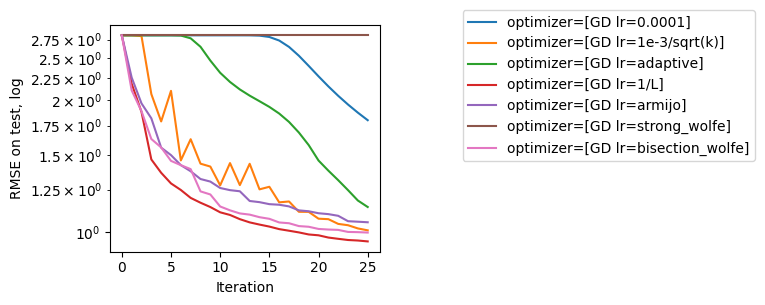
\includegraphics[width=\textwidth,keepaspectratio]{../data/gd.png}
  \caption[Gradient descent]{Gradient descent (\Cref{algo:gd})}\label{fig:gd}
\end{figure}

\begin{figure}[H]
  \centering
  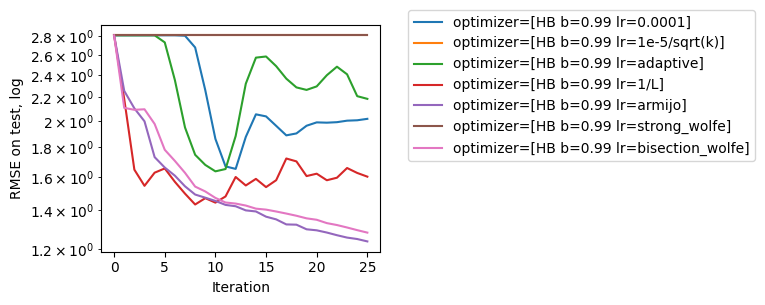
\includegraphics[width=\textwidth,keepaspectratio]{../data/hb.png}
  \caption[Heavy Ball]{Heavy Ball (\Cref{algo:hb})}\label{fig:hb}
\end{figure}

\begin{figure}[H]
  \centering
  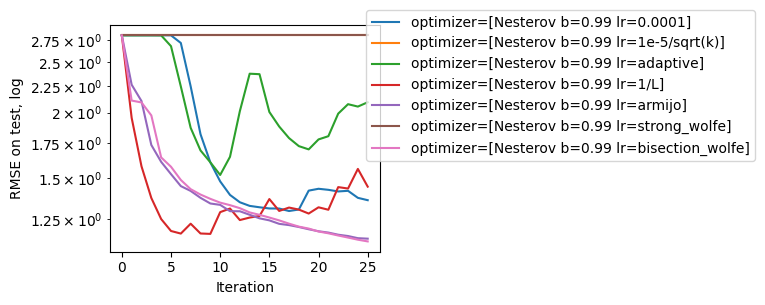
\includegraphics[width=\textwidth,keepaspectratio]{../data/Nesterov.png}
  \caption[Nesterov]{Nesterov Accelerated  Gradient (\Cref{algo:nesterov})}\label{fig:nesterov}
\end{figure}

\begin{figure}[H]
  \centering
  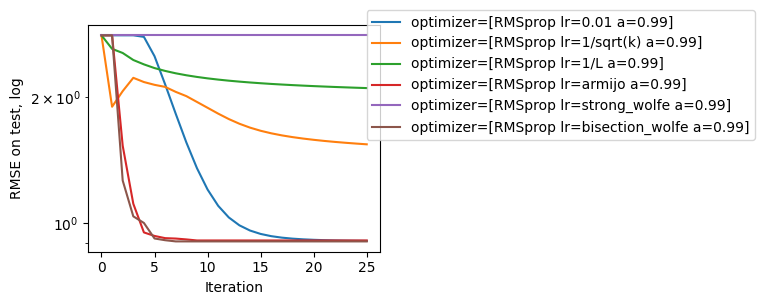
\includegraphics[width=\textwidth,keepaspectratio]{../data/rmsprop.png}
  \caption[RMSProp]{RMSProp (\Cref{algo:rmsprop})}\label{fig:rmsprop}
\end{figure}

\begin{figure}[H]
  \centering
  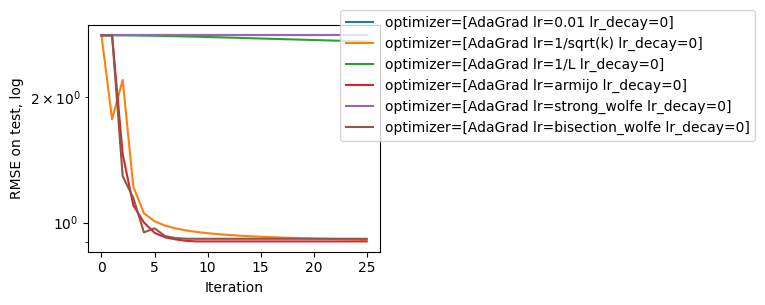
\includegraphics[width=\textwidth,keepaspectratio]{../data/adagrad.png}
  \caption[AdaGrad]{AdaGrad (\Cref{algo:adagrad})}\label{fig:adagrad}
\end{figure}

\begin{figure}[H]
  \centering
  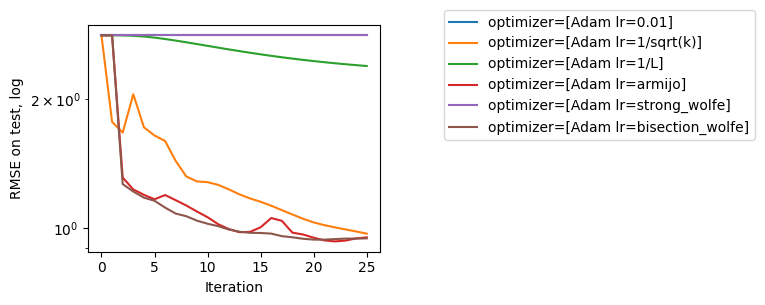
\includegraphics[width=\textwidth,keepaspectratio]{../data/adam.png}
  \caption[Adam]{Adam (\Cref{algo:adam})}\label{fig:adam}
\end{figure}

\begin{figure}[H]
  \centering
  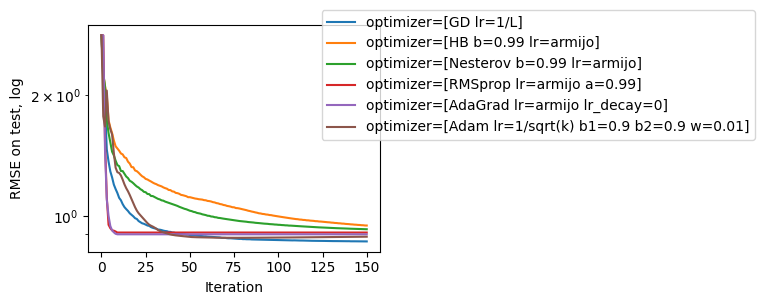
\includegraphics[width=\textwidth,keepaspectratio]{../data/comparison.png}
  \caption[Comparison]{Comparison of optimizers with best configurations}\label{fig:comparison}
\end{figure}

\begin{figure}[H]
  \centering
  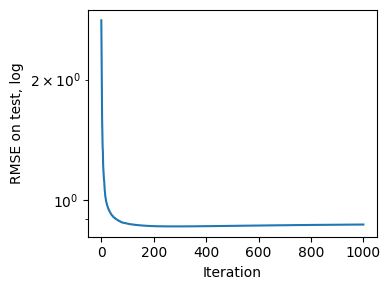
\includegraphics[keepaspectratio]{../data/final.png}
  \caption[Best model]{Best model: $r=10$, Gradient Descent with estimate 1/L strategy and $\lambda=2$}\label{fig:best}
\end{figure}

\begin{figure}[H]
  \centering
  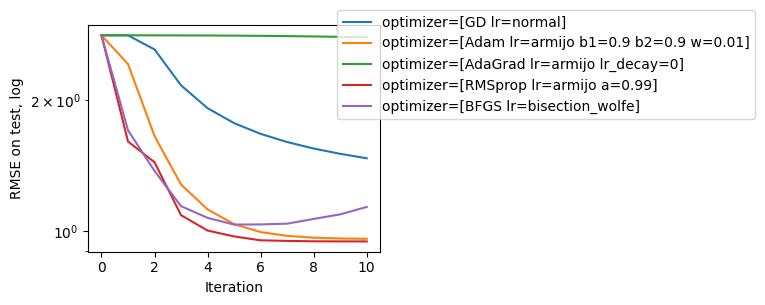
\includegraphics[width=\textwidth,keepaspectratio]{../data/vector_gd.png}
  \caption[Vector GD]{Vector Gradient Descent}\label{fig:vector_gd}
\end{figure}

\begin{figure}[H]
  \centering
  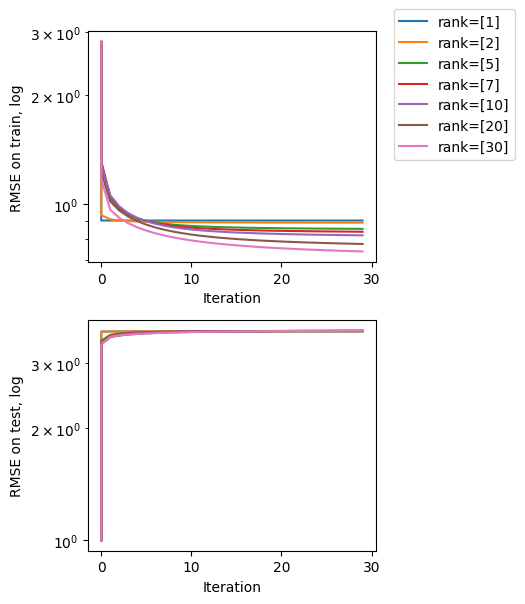
\includegraphics[keepaspectratio, scale=0.7]{../data/nnmf.png}
  \caption[NNMF]{Non-Negative Matrix Factorization}\label{fig:nnmf}
\end{figure}

\end{document}
